% IMPORTANT! In order for the document to compile, one needs to use XeLaTeX or LuaLaTeX as compiler. This can be done in  Overleaf by Menu -> Settings -> Compiler -> Choose XeLaTeX/LuaLaTeX
\documentclass[12pt]{article}

\usepackage{KUstyle}
\usepackage[margin=0.8in]{geometry} 
\usepackage{setspace} % Package for linespacing
\usepackage{tabularx} % Package for table
\usepackage{fontspec}
\usepackage{amsmath}
\usepackage{fontspec}
\usepackage{listings}
\usepackage{xcolor}
\usepackage{graphicx}
\usepackage{forest}
\usepackage{float}
\setlength{\parindent}{0pt}
\usepackage[normalem]{ulem} % for \sout
\usepackage{algorithm}
\usepackage{algpseudocode}
\usepackage{tikz}
\usepackage{pdfpages}


\lstset{
  basicstyle=\ttfamily\small,
  keywordstyle=\color{blue},
  stringstyle=\color{orange},
  commentstyle=\color{gray},
  showstringspaces=false,
  breaklines=true,
  frame=single
}




% This change the content of the frontpage
\ptype{Bachelors project}
\author{Carl-Emil Rohde og Emil Oliver Olesen}
\title{Constraint-based Scheduling in CP-SAT}
\date{Date: {June 2025}}
\advisor{Advisor: {Thomas Hildebrandt}}
\fpimage{billede3.png} % Remove this command if no image is desired





\begin{document}




\maketitle




\onehalfspacing


\begin{table}[h]
\def\arraystretch{1.5}
\begin{tabularx}{\textwidth}{l X}
Institute: & {University Of Copenhagen}  \\
Department & {Department for Computer Science} \\
Author(s): & {Carl-Emil Rohde (kvb125), Emil Oliver Olesen(fps618)} \\
Title and subtitle: & {Constraint scheduling} \\
Description: & A project examining the use of constraint programming resource allocation problems for soccer clubs \\
Advisor: & {Thomas Hildebrandt} \\
Date: & 10 06 2025
\end{tabularx}
\end{table}


\section*{Explore Our Scheduling Tool}


\begin{itemize}
    \item \textbf{Introduction Video (danish):} \url{https://youtu.be/YgxFKXcI10I}
    \item \textbf{Webpage:} \url{https://baneplanen.info/}
    \item \textbf{GitHub Repository:} \url{https://github.com/rohde01/field-schedule.git}
\end{itemize}




\newpage


\begin{abstract}
This project investigates the applicability of constraint programming, specifically using Google's CP-SAT solver, to the scheduling of football training sessions in grassroots clubs. The core challenge lies in allocating a limited set of divisible field resources to multiple teams over a constrained weekly time grid, while satisfying hard constraints and optimising for preferences such as training spread and team co-location.

We model the problem using discrete time slots, hierarchical fields, and global constraints such as \texttt{NoOverlap} and \texttt{Cumulative}, enabling strong propagation. A case study based on real club data demonstrates that CP-SAT finds high-quality solutions efficiently, even under near-maximal utilisation. In the largest instance, a feasible solution is found in 3.6 seconds, and a near-optimal one within two minutes.

While the model performs well in discrete domains, it is sensitive to objective weight calibration and less suited to continuous or dynamic scheduling contexts. Nonetheless, the results show that constraint programming offers a scalable and interpretable framework for structured real-world planning problems.
\end{abstract}

\newpage


\renewcommand{\contentsname}{Table of content}


\tableofcontents
\newpage


\newpage


\section{Introduction}

Every week, grassroots soccer clubs across the country face a surprisingly complex logistical task: allocating limited field time to a growing number of youth and senior teams. Fields must be shared fairly, practices should be spaced sensibly throughout the week, and younger age groups often require smaller playing areas or earlier time slots. On top of this, some clubs operate facilities where full-size fields can be divided into halves or quarters, further complicating the allocation process. What might at first glance seem like a simple calendar exercise quickly becomes a puzzle of interdependent constraints, scarce resources, and diverging preferences.

Many clubs solve this puzzle manually, often relying on spreadsheets, experience, and compromise. While this approach is familiar, it has several downsides: it is time-consuming, lacks transparency, and often fails to fully meet teams' needs. Even small errors or oversights can cause inefficiencies or lead to dissatisfaction among coaches and players. In this context, more structured, rule-based approaches become increasingly attractive.
\\

\textbf{This project} explores whether constraint-based scheduling, an approach grounded in logic and mathematics, can offer a better solution. Specifically, we investigate whether modern constraint programming tools, such as Google's CP-SAT solver, can handle the real-world complexity of soccer club scheduling. These tools allow rules and preferences to be defined declaratively, such as "teams should not train more than two days in a row" or "younger teams should not train after 7 PM"-and then automatically search for solutions that satisfy all hard requirements while optimising for softer goals like fairness and co-location.
\\
\\
\textbf{We focus} on a particularly rich variant of the problem: how to schedule practices when fields can be subdivided hierarchically (e.g., from full to half to quarter fields), and when multiple, sometimes competing, objectives must be considered. To evaluate this approach, we design and implement a scheduling model tailored to a real club scenario, and use it to investigate the capabilities and limitations of constraint programming in this setting.

In doing so, the project aims not only to improve a specific planning problem but also to highlight how constraint-based scheduling can serve as a general and transparent tool for for other relevant branches.
\newpage



\subsection{Research questions}
\bullet{RQ1:} How can CP (CP-SAT) model the combinatorial structure of a real-world, subdivisible-field scheduling problem?
\\
\bullet{RQ2:} How do modelling strategies, along with the formulation of constraints and variables, influence the quality of solutions and the efficiency of solving constraint programming models?



\section{Case study}

\subsection{Context.}
A football club manages a collection of playing areas $\mathcal{F}$, which can be used either as full-size fields or subdivided hierarchically into halves and quarters. Each (sub)field $f \in \mathcal{F}$ is defined by the following characteristics:
\\

\begin{tabular}{@{}ll@{}}
\textbf{Type:} & $t(f) \in \{\text{full}, \text{half}, \text{quarter}\}$ \\
\textbf{Nominal size:} & $s(f) \in \{11 \times 11,\; 8 \times 8,\; 5 \times 5,\; 3 \times 3\}$ \\
\textbf{Capacity weight:} & $c(f) \in \{1000,\; 500,\; 250,\; 125\}$, halved at each subdivision \\
\end{tabular}
\\

When a field is allocated to a session, all of its subfields become unavailable for that time slot, and the same holds in reverse: if a subfield is in use, its parent field is also unavailable.
\\

\textbf{Self referencing field schema}
\begin{lstlisting}[language=Python]
class Field(BaseModel):
    field_id: int = Field(gt=0)
    size: FieldSize
    field_type: FieldType
    parent_field_id: Optional[int] = None
    availability: Dict[DayOfWeek, FieldAvailability]
    quarter_subfields: List[SubField] = []
    half_subfields: List[SubField] = []

\end{lstlisting}

\vspace{.5\baselineskip}
\subsection{Temporal discretisation}

The weekly planning horizon $\mathcal{T}$ is divided into fixed 15-minute time slots. Each slot is indexed by a pair $(d,\tau)$, where $d \in \{0, \dots, 6\}$ represents the day of the week, and $\tau$ denotes the intra-day slot index.

\subsection{Training session requests}

The input includes a set of training session requests $\mathcal{R}$, where each request $r \in \mathcal{R}$ is defined by the following attributes:
\\

\begin{tabular}{@{}ll@{}}
\textbf{Team identifier:} & $\mathrm{team}(r)$ \\
\textbf{Team year:} & $\mathrm{year}(r)$ \\
\textbf{Session length:} & $\ell(r)$, in 15-minute slots \\
\textbf{Fixed start time:} & Optional $(d^{\!*}(r), \tau^{\!*}(r))$ \\
\textbf{Fixed field:} & Optional $f^{\!*}(r)$ \\
\textbf{Capacity demand:} & Required $C^{\!*}(r) \in \{125,\; 250,\; 500,\; 1000\}$ if no fixed field is given \\
\end{tabular}
\\

If any of the attributes, day, time, or field are fixed, they act as hard constraints. If omitted, the optimiser is free to assign suitable values within the allowed bounds.
\\

\textbf{Constraint schema}
\begin{lstlisting}[language=Python]
class Constraint(BaseModel):
    uid: UUID
    team_id: int
    year: str = Field(pattern=r'^U([4-9]|1[0-9]|2[0-4])$')
    start_time: Optional[str] = Field(None, pattern=r'^([01]\d|2[0-3]):([0-5]\d)$')  # HH:MM format
    length: int
    day_of_week: Optional[Literal[0, 1, 2, 3, 4, 5, 6]] = None
    required_cost: Optional[Literal[125, 250, 500, 1000]] = None
    field_id: Optional[int] = None
\end{lstlisting}


\vspace{.5\baselineskip}
\subsection{Feasibility constraints.}
A schedule is \emph{feasible} if
\begin{enumerate}
  \item no session overlaps itself: a request occupies $\ell(r)$
        consecutive slots;
  \item no two sessions overlap on the same (sub)field or any of its
        ancestors/descendants;
  \item whenever $f^{\!*}(r)$ is specified, $r$ is placed on that field;
  \item whenever $(d^{\!*}(r),\tau^{\!*}(r))$ is specified, $r$ begins
        exactly then;
    \item if only $C^{\!*}(r)$ is specified, $r$ must be assigned to
          some $f$ with $c(f)\!\ge\!C^{\!*}(r)$;
          the values $1000,500,250,125$ correspond respectively to
          full, half and quarter fields.

\end{enumerate}

\vspace{.5\baselineskip}
\subsection{Multi objective criteria.}
Among all feasible schedules we seek one that:
\begin{itemize}
  \item[\textbf{O1}] \emph{minimises} the longest chain of consecutive training days experienced by any team:  
        $\displaystyle\min\bigl(\max_{k\in\mathcal{K}}L_k\bigr)$;
  \item[\textbf{O2}] \emph{maximises} the co‑location of teams from the same age category within the same main field during the same time slot:  
        $\displaystyle\max\!\sum_{y,\sigma,m}\binom{n_{y,\sigma,m}}{2}$;
\end{itemize}


\vspace{.5\baselineskip}
\subsection{Goal.}
The case study investigates the suitability of
\emph{constraint‑based scheduling} techniques, backtracking search,
branch‑and‑bound, global constraints, and tailored heuristics for
constructing schedules that satisfy the above hard constraints while
optimising (O1)–(O2).  A CP‑SAT prototype for the described football‑field
allocation problem serves as the concrete evaluation vehicle.




\section{Theoretical foundation}



\subsection{Definition and Core Idea of CP}

Constraint Programming (CP) is a programming paradigm widely applied to solving complex combinatorial problems, particularly where resources are limited or constrained. This scenario frequently occurs across diverse practical contexts in our daily lives, such as allocating classrooms to classes in educational institutions, managing beds and facilities in hospitals, or optimizing field scheduling in football clubs to maximize resource utilization among numerous teams.

\vspace{0.5em}
\noindent
Beginning with a simple model focused on field scheduling within a football club, we can identify common characteristics shared across such constraint problems and categorize them into three fundamental components: Variables, Domains, and Constraints.

\begin{equation}
\label{eq:csp_definition}
\begin{aligned}
X &: \text{A set of variables, } \{X_1, X_2, \dots, X_n\} \\
D &: \text{A set of domains for each } X_i,\; \{D_1, D_2, \dots, D_n\} \\
C &: \text{A set of constraints}
\end{aligned}
\end{equation}


\vspace{0.5em}
\noindent
\textbf{Variables} represent the decisions or choices that the model must determine. Initially unknown, these might include which specific field a team should train on and at what specific time.

\vspace{0.5em}
\noindent
\textbf{Domains} define the set of possible values that each variable can assume. Typically, these domains are discrete, as exemplified in this context by fixed fields and predefined available time slots.

\vspace{0.5em}
\noindent
\textbf{Constraints} are rules or conditions that must be satisfied by the chosen variable assignments, effectively narrowing the solution space. An evident constraint within such scheduling problems would be ensuring that no two teams are allocated the same field simultaneously, thus avoiding overlapping schedules.

\vspace{0.5em}
\noindent
In some contexts, all feasible solutions may be considered equally acceptable. However, in other cases, the usefulness of a solution can vary depending on subjective preferences or contextual factors, requiring the model to incorporate soft constraints to express these nuances. If all valid solutions are considered equally desirable, the problem can be formulated as a Constraint Satisfaction Problem (CSP).

\vspace{0.5em}
\noindent
As a simple example, consider a football club with two teams (A and B) and one field (Field 1), which is available for two one-hour time slots (17:00–18:00 and 18:00–19:00). Each team must be assigned a training session on the field, and no two teams can use the field at the same time.

\vspace{0.5em}
\noindent
The corresponding CSP model, illustrated by the decision tree in Figure~\ref{fig:csp_2teams_1field}, can be formally defined as a triple $(X, D, C)$, where:

\begingroup
\setlength{\jot}{5pt}
\begin{equation}
\label{eq:csp_2teams}
\begin{aligned}
X &= \{X_A, X_B\} 
&& \text{each variable } X_i \text{ assigns a timeslot to team } i \\
D &= \{D_A, D_B\} 
&& \text{with } D_i = \{17{:}00, 18{:}00\} \text{ for each team} \\
C &= \left\{ (X_A, X_B) \mid X_A \neq X_B \right\} 
&& \text{no two teams can train at the same time on the same field}
\end{aligned}
\end{equation}
\endgroup




\begin{figure}[H]
\centering
\begin{forest}
for tree={
    draw,
    rounded corners,
    node options={align=center, inner sep=4pt},
    l sep=15pt,
    s sep=6pt,
    edge={->,>=latex}
}
[Start
  [A: 17:00
    [B: 17:00\\(Conflict) $\times$]
    [B: 18:00\\(Valid) $\checkmark$]
  ]
  [A: 18:00
    [B: 17:00\\(Valid) $\checkmark$]
    [B: 18:00\\(Conflict) $\times$]
  ]
]
\end{forest}
\caption{CSP example.}
\label{fig:csp_2teams_1field}
\end{figure}

\vspace{0.5em}
\noindent
As can be easily verified, the CSP instance presented above admits two feasible solutions. We initially assume that it is irrelevant whether Team A trains from 17:00–18:00 or from 18:00–19:00; the only constraint is that Team B must train in the time slot not used by Team A. 

\vspace{0.5em}
\noindent
However, let us now assume that training time is not entirely indifferent. Suppose Team B consists of younger players who prefer to train earlier in the day. In this case, we may wish to extend our model to include \textit{soft constraints}, such as preferences, and reformulate it as a \textit{Constraint Optimization Problem (COP)}, where we honor the model points, based on how well it meets our soft constraints.

\begin{equation}
\label{eq:cop_model}
\begin{aligned}
f(X) &= 
\begin{cases}
1 & \text{if } X_B = 17{:}00 \\
0 & \text{otherwise}
\end{cases}
&& \text{objective: reward early training for Team B}
\end{aligned}
\end{equation}

\begin{figure}[H]
\centering
\begin{forest}
for tree={
    draw,
    rounded corners,
    node options={align=center, inner sep=4pt},
    l sep=15pt,
    s sep=6pt,
    edge={->,>=latex}
}
[Start
  [A: 17:00
    [B: 17:00\\(Conflict) $\times$]
    [B: 18:00\\(Valid) $\checkmark$\\Score: 0]
  ]
  [A: 18:00
    [B: 17:00\\(Valid) $\checkmark$\\Score: 1]
    [B: 18:00\\(Conflict) $\times$]
  ]
]
\end{forest}
\caption{Constraint Optimization Problem (COP)}
\label{fig:cop_tree_2teams}
\end{figure}





\vspace{1.5em}
\noindent
The new COP model still finds two valid solutions, but one is more desirable than the other because the score is higher when Team B’s training session starts at 17:00. This simple setup with two teams, one field, and two time slots makes it relatively easy to find feasible solutions, even with a few hard and soft constraints. However, one can quickly realize how the complexity of the problem scales dramatically with even small increments in variables, resources, and constraints.

\vspace{1em}
\noindent
\textbf{Example on how complexity scales}

Consider first a simple case with two teams (A and B), one field, and two time slots. Each team must train once, and the field can only be used by one team at a time. Without constraints, there are:

\begin{equation}
|D_A| \times |D_B| = 2 \times 2 = 4
\end{equation}

Imposing the non-overlap constraint reduces this to: $2\times 1$
\\

Now extend the scenario to three teams, two fields, and three time slots. Ignoring constraints, each team has 6 options (2 fields × 3 slots), giving:

\begin{equation}
6^3 = 216
\end{equation}

Introducing the same non-overlap rule, the feasible combinations drop to: $6 \times 5 \times 4 = 120$
\\

Even this small increase in problem size causes a rapid growth in the solution space. Adding soft preferences such as field or time priorities further transforms the problem from a simple CSP into a complex COP, where optimisation techniques are needed to efficiently identify good solutions.




\subsection{Variable types in CP}

Constraint Programming (CP) derives its flexibility and efficiency from a diverse set of variable abstractions, each tailored to represent different aspects of a decision problem. In CP–SAT, integer, Boolean, and interval variables coexist in one solver, allowing us to model the football‐field scheduling problem in a natural and concise way. Below, we summarise these variable types, explain their role in our model, and highlight the advantages they provide over a purely linear or SAT‐based formulation.

\paragraph{Integer variables.}
An integer variable $x$ represents a choice drawn from a finite set of integers, typically written as
\[
  x \in \mathbb{Z} \cap [L,U],
\]
where $L$ and $U$ are known bounds. In our scheduling context, we introduce a start‐slot index
\[
  \tau(r) \in \{0,\dots,|\mathcal T|-1\}
\]
for each request $r$, which determines when a session begins in units of 15‐minute time slots. We create one integer variable for each potential assignment (request, resource, day) to represent its start and end times, with domains restricted by each field’s availability window. Rather than modelling splitting decisions as solver variables, we precompute all subfield resources and their capacities, and enforce capacity limits via a cumulative constraint on the set of intervals corresponding to a top‐level field.

\paragraph{Boolean indicator variables.}
Whenever a decision is binary, such as “does session $r$ run on subfield $f$ on day $d$?”, we introduce a Boolean variable
\[
  y_{r,f,d} \in \{0,1\}.
\]
We enforce that each session is assigned exactly once via
\[
  \sum_{f,d} y_{r,f,d} = 1 \quad (\forall r),
\]
and let these Booleans control presence or absence of the corresponding time intervals. Mutual exclusion of overlapping sessions on the same resource is enforced by interval and global constraints, rather than pairwise Boolean clauses, and teams are restricted to at most one session per day by
\[
  \sum_{f} y_{r,f,d} \le 1 \quad (\forall \text{team},\,\forall d).
\]
Boolean propagation and clause learning in CP–SAT further prune infeasible assignments early.

\paragraph{Interval variables.}
When sessions span multiple consecutive slots, we bundle start, duration, and end into an interval variable:
\[
  I_{r,f,d} = [\mathrm{start},\,\mathrm{end}),
\quad
\mathrm{end} = \mathrm{start} + \ell(r),
\]
with presence indicator $y_{r,f,d}$. For each potential assignment we create an optional interval, and post a NoOverlap constraint across intervals on the same resource (and across ancestor/descendant resources), as well as a cumulative capacity constraint on the top‐level field:
\[
  \text{AddNoOverlap}(\{I_{r,f,d}\})
  \quad
  \text{and}
  \quad
  \text{AddCumulative}(\{I\},\{\text{demand}\},\text{capacity}).
\]
Advanced filtering algorithms like edge‐finding aggressively narrow start‐time domains, synchronizing “where” and “when” choices via the presence Booleans.

Together, these three variable types capture time‐based decisions (integers), discrete assignments (Booleans), and scheduling blocks (intervals) in a unified model that outperforms pure MILP or SAT encodings.


\subsection{Common Constraint Types}

Once variables are declared, CP–SAT requires a collection of constraints to bind them. In our football scheduler, five families of constraints capture the essential hard requirements. Thanks to OR-Tools’ highly optimised implementations, each global constraint not only encodes logical or arithmetic relations concisely but also provides strong propagation that cuts down the search tree dramatically.

\paragraph{Set-partitioning constraints.}
For each request \(r\in\mathcal{R}\), we have a set of Boolean indicators \(\{y_{r,f,d}\mid f\in\mathcal{F},\,d\in\{0,\dots,6\}\}\) over all eligible fields and days. The requirement that “each session is scheduled exactly once” is enforced by the linear equation
\[
  \sum_{f,d} y_{r,f,d} = 1
  \quad(\forall r\in\mathcal{R}).
\]
In OR-Tools, the routine \texttt{AddExactlyOne(...)} implements this in a single call. As soon as one literal \(y_{r,f,d}=1\) is set, all other \(y_{r,f',d'}\) for the same \(r\) are forced to 0. This instantaneous pruning is far stronger than posting \(\binom{n}{2}\) pairwise inequalities, especially when \(r\) has many potential \((f,d)\) pairs.

\paragraph{Disjunctive constraints.}
A disjunctive constraint ensures that two activities sharing a common resource do not overlap in time. In our model, for any given subfield \(f\) on a specific day \(d\), we collect all optional intervals \(\{I_{r,f,d}\mid r\in\mathcal{R}\}\) and post
\[
  \texttt{NoOverlap}\bigl(\{I_{r,f,d}\}_{r}\bigr),
\]
so no two intervals can overlap. To enforce hierarchical conflicts, i.e., if a parent field is used, none of its children may be used at overlapping times we also post a NoOverlap constraint on the union of intervals belonging to any ancestor–descendant pair \((f_{\text{parent}},\,f_{\text{child}})\). Because NoOverlap performs edge-finding and not-first/not-last filtering, it can detect, for instance, that if a long session is placed at midday, two shorter sessions cannot both fit around it. This global awareness is more powerful than writing disjunctions of the form “\(\text{end}(I)\le\text{start}(J)\) or \(\text{end}(J)\le\text{start}(I)\)” for every pair, since it reasons simultaneously over all intervals on that resource.


\paragraph{Cumulative resource constraints.}
A top-level field \(F\in\mathcal{F}\) can host multiple simultaneous quarter or half field sessions, provided the sum does not exceed main field capacity. Define for every \((r,f,d)\) the integer demand
\[
  d_{r,f} =
  \begin{cases}
    1000 \\
    500 \\
    250 \\
    125 \\
  \end{cases}
\]
whenever \(y_{r,f,d}=1\). Then for each top field \(F\) and each day \(d\), we gather all intervals \(I_{r,f,d}\) under \(F\) (including children and grandchildren) and invoke
\[
  \texttt{AddCumulative}\bigl(\{(I_{r,f,d},\,d_{r,f}) \mid f \trianglelefteq F,\;r\in\mathcal{R}\},\,c(F)\bigr).
\]
This global constraint enforces that, at every time point \(t\),
\[
  \sum_{\substack{r,f:\\I_{r,f,d}\ni t}} d_{r,f} \le c(F).
\]
The AddCumulative propagator tracks the running load on \(F\) and prunes any start time \(\tau\) for which there exists a subset of overlapping demands whose sum exceeds \(c(F)\). Modeling this with linear constraints alone would require discretising time or introducing auxiliary variables, resulting in a far larger and weaker model.

\paragraph{Cardinality and at-most-one constraints.}
To enforce that each team \(k\) cannot train more than once per day, we gather all Booleans \(\{y_{r,f,d}\mid \mathrm{team}(r)=k,\;f\in\mathcal{F}\}\) for a fixed team \(k\) and day \(d\), and post the inequality
\[
  \sum_{r:\mathrm{team}(r)=k}\sum_{f} y_{r,f,d} \le 1.
\]
Although weaker than a global scheduling constraint, this still tightens the search because, once any \(y_{r,f,d}=1\) is set, all other Booleans for that team and day must be 0. Combined with other constraints, such as cumulative capacity, this early pruning quickly rules out infeasible assignments.

\paragraph{Reified and conditional constraints.}
Some requests include fixed start times \((d^*(r),\tau^*(r))\) or fixed fields \(f^*(r)\). To model statements such as “if request \(r\) is placed on field \(f^*(r)\) at day \(d^*(r)\), then its start time must be exactly \(\tau^*(r)\); otherwise that assignment is disallowed,” we use reification via the OnlyEnforceIf mechanism:
\[
  y_{r,f^*,d^*} = 1 \Longrightarrow \text{start}(I_{r,f^*,d^*}) = \tau^*(r),
\]
and if \(\tau^*(r)\) lies outside the availability window \([\text{ws},\,\text{we}-\ell(r)]\) for that field and day, then
\[
  \tau^*(r)\not\in[\text{ws},\,\text{we}-\ell(r)]
  \Longrightarrow y_{r,f^*,d^*} = 0.
\]
Reification links a Boolean with a linear equality or inequality, so if the fixed time falls outside the window, the presence Boolean is immediately forced to 0. Conversely, if the solver sets the Boolean to 1, then the start-time equality is enforced without further search. This direct coupling is far more efficient than adding large numbers of big-\(M\) linear constraints.

\bigskip

Taken together, these five families, ExactlyOne, NoOverlap, Cumulative, cardinality/at-most-one, and reified constraints, form the backbone of our CP model. Each corresponds crisply to a piece of the football-field allocation logic: ExactlyOne ensures each session picks one \((f,d)\); NoOverlap enforces that no two sessions share the same turf simultaneously, respecting both partitioned subfields and parent–child hierarchies; Cumulative guards the aggregate capacity of each top-level field; cardinality constraints prevent a team from appearing more than once per day; and reified constraints immediately satisfy or discard fixed-time/field requests. By deploying these global constraints rather than only pairwise or big-\(M\) constraints, CP–SAT achieves much stronger domain reduction before and during search, which is essential for scaling to dozens of teams, hundreds of sessions, and multi-level field hierarchies.


\subsection{Constraint solving with \texttt{CP--SAT}}
\label{sec:cp_sat_solver}

After defining variables and assembling the five families of global constraints, the next step is to solve the resulting model to find a feasible or optimal schedule. Google’s CP–SAT solver is a state-of-the-art hybrid engine that merges classic CP propagation with SAT-style clause learning and branch-and-bound for optimisation. In the following, we outline the key algorithmic components, emphasising how each feature is leveraged in our football scheduling problem.
\\
\\
The search process in CP–SAT can be understood as a decision tree, where each node represents a partial assignment, for example, assigning a training session to a field on a specific day. Without pruning, the solver would explore the full combinatorial space. However, as soon as a partial assignment leads to a violation of hard constraints such as overlapping sessions or insufficient field capacity the entire branch is discarded, including all its subbranches.

\begin{figure}[H]
\centering
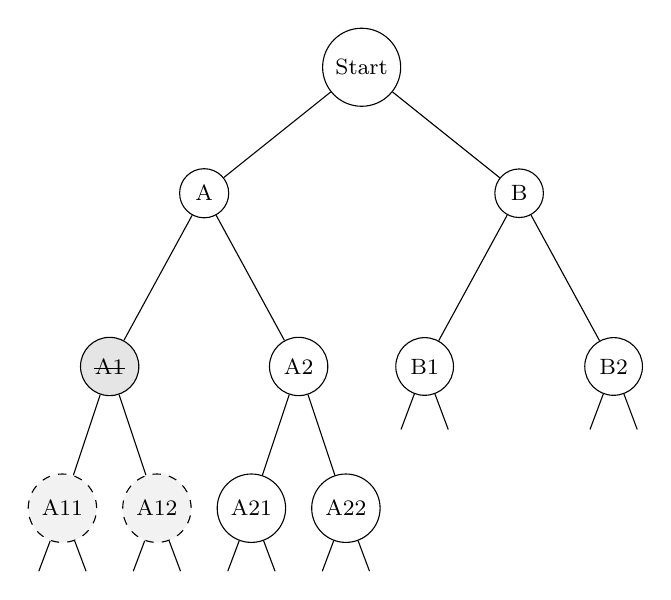
\begin{tikzpicture}[
  level 1/.style={sibling distance=4cm, level distance=1.6cm},
  level 2/.style={sibling distance=2.4cm, level distance=2.2cm},
  level 3/.style={sibling distance=1.2cm, level distance=1.8cm},
  every node/.style={font=\footnotesize},
  pruned/.style={circle,draw,fill=gray!20},
  faint/.style={circle,draw,dashed,fill=gray!10}
]

\node[circle,draw]{Start}
  child {node[circle,draw]{A}
    child {node[pruned]{\sout{A1}}
      child {node[faint](a11){A11}}
      child {node[faint](a12){A12}}
    }
    child {node[circle,draw]{A2}
      child {node[circle,draw](a21){A21}}
      child {node[circle,draw](a22){A22}}
    }
  }
  child {node[circle,draw]{B}
    child {node[circle,draw](b1){B1}}
    child {node[circle,draw](b2){B2}}
  };

\foreach \n in {a11,a12,a21,a22,b1,b2} {
  \draw (\n) -- ++(-0.3,-0.8);
  \draw (\n) -- ++(0.3,-0.8);
}

\end{tikzpicture}
\caption{Pruning of infeasible subtrees in the CP–SAT decision tree.}
\end{figure}

Figure 3 illustrates how CP–SAT avoids traversing infeasible parts of the search space. In this example, once the solver reaches node A1 and detects a conflict (for example, overlapping sessions or invalid capacity), the entire subtree below A1 is discarded. This aggressive pruning mechanism can eliminate thousands of combinations in a single step.

\subsubsection*{Constraint propagation loop}
At its core, CP–SAT repeatedly executes a propagation loop that maintains reduced domains for all variables whenever a new assignment is made:
\[
  \text{(propagation)} \;\longrightarrow\;\text{(domain pruning)} \;\longrightarrow\;\text{(repeat until fixpoint or conflict)}.
\]
During this loop, whenever a Boolean or integer is assigned, each active global constraint wakes up and tightens the domains of its associated variables. For example, if a presence literal \(y_{r,f,d}=1\) is fixed, \texttt{AddExactlyOne} immediately sets all other \(y_{r,f',d'}\) for the same \(r\) to 0, which in turn triggers interval-related propagators to restrict start times. Similarly, \texttt{AddNoOverlap} performs edge-finding and not-first/not-last filtering on optional intervals, pruning start domains when the remaining free time on a field becomes too short. Meanwhile, \texttt{AddCumulative} builds a partial demand profile over each top field’s time horizon and removes any start times that would cause the running sum of demands to exceed capacity. Conditional propagators attached via \texttt{OnlyEnforceIf} immediately enforce or discard fixed start-time or fixed-field requirements. These propagators iterate until no further domain changes occur (a fixpoint) or a variable’s domain becomes empty, at which point a conflict is detected and the solver learns a nogood clause.

\subsubsection*{Lazy-clause generation and nogood learning}
When propagation alone cannot rule out a partial assignment but later finds that no extension can satisfy all constraints, CP–SAT generates a nogood clause, a Boolean disjunction that captures why the combination of decisions is infeasible. For instance, if \(y_{r,f,d}=1\) and \(y_{r',f,d}=1\) but their corresponding intervals overlap, the solver learns the clause
\[
  \neg(y_{r,f,d}=1)\;\lor\;\neg(y_{r',f,d}=1),
\]
preventing any future branch from assigning both to 1. Because many subfields are structurally identical, such as all quarter-fields of the same top-level pitch, a single learned clause can prune an entire class of symmetric assignments. This mechanism, known as lazy clause generation, injects learned clauses into an underlying CDCL SAT core and enables backjumping to the earliest decision level where the conflict can be avoided. As a result, the solver never repeats an infeasible partial assignment and significantly reduces redundant search.

\subsubsection*{Branching heuristics and value selection}
After propagation reaches a fixpoint with no conflict and not all variables are assigned, CP–SAT selects a decision literal using a VSIDS-like heuristic. It maintains activity scores for all unassigned Booleans based on how often they have appeared in recent conflicts. In our model, presence Booleans \(y_{r,f,d}\) typically dominate these scores, since many conflicts revolve around resource contention. By selecting the most entangled \(y_{r,f,d}\) first, the solver focuses on the critical assignments that will prune the largest portion of the tree. For a chosen Boolean \(y_{r,f,d}\), the solver first tries
\[
  y_{r,f,d} = 1,
\]
i.e., assign session \(r\) to \((f,d)\), and only if that fails does it try
\[
  y_{r,f,d} = 0.
\]
For integer variables, CP–SAT splits the domain \([L,U]\) into two halves \([L,M]\) and \([M+1,U]\), exploring one branch before the other. Since we solve an optimisation problem via \texttt{Minimize}, CP–SAT employs branch-and-bound: whenever a complete assignment satisfies all constraints, the solver records its objective value as the current best, then prunes any partial assignment whose bound cannot surpass the incumbent. In practice, this means that once a good feasible schedule is found quickly, further search focuses on improving the objective rather than rediscovering a feasible solution.


\subsection{Multi‐Objective Optimisation}

In many realistic scheduling scenarios, a single criterion is insufficient to capture all desirable aspects of a solution. In our football‐field allocation problem, we identified two qualitatively distinct objectives:
\[
\begin{aligned}
\textbf{O1:}\;& \text{Minimise the longest chain of consecutive training days for each team, then sum over all teams;}\\
\textbf{O2:}\;& \text{Minimise the year‐gap among teams sharing the same top‐level field on the same day.}
\end{aligned}
\]
Taken individually, each criterion yields a preference ordering over feasible schedules. Together, however, they induce a multi‐objective optimisation problem. In this section, we first formalise the multi‐objective setting and then describe how CP–SAT can accommodate these two goals in a single solve.

\paragraph{Lexicographic and weighted‐sum approaches.}
A common technique to handle multiple objectives is to combine them into a single scalar objective via a weighted sum:
\[
\min\; w_1\,O_1 + w_2\,O_2,
\]
where the weights \(w_1\) and \(w_2\) reflect the relative importance of each criterion. However, when one objective must never be sacrificed for the sake of another (a strict lexicographic ordering), we can simulate this by choosing one weight much larger than any possible value of the second term:
\[
\min\; O_1 \times M + O_2,
\]
where \(M\) exceeds the maximum attainable value of \(O_2\). This ensures the solver first optimises \(O_1\) to its minimum, and only then tightens \(O_2\) without backtracking on \(O_1\).

\paragraph{Implementation in CP–SAT.}
OR‐Tools’ CP–SAT solver supports a single linear minimisation objective, so we encode our two‐stage optimisation by constructing a composite objective expression within the model:
\[
  \mathrm{Obj} \;=\; 
  \begin{cases}
    \texttt{adjacency\_obj} \times M \;+\;\texttt{year\_gap\_obj}, & \text{if both objectives are enabled},\\
    \texttt{adjacency\_obj}, & \text{if only the weekday‐chain objective is enabled},\\
    \texttt{year\_gap\_obj}, & \text{if only the year‐gap objective is enabled}.
  \end{cases}
\]
In our implementation we choose \(M=100\), which safely exceeds the maximum possible sum of age‐category gaps across all fields and days. The code fragment is:
\begin{verbatim}
if request.weekday_objective and request.start_time_objective:
    model.Minimize(adjacency_objective * 100 + objectives[1])
elif objectives:
    model.Minimize(sum(objectives))
\end{verbatim}

The lexicographic scheme guarantees that any improvement in the primary objective \(O_1\) cannot be offset by a worsening of \(O_2\). This aligns well with scenarios where, for example, minimising consecutive training days is deemed strictly more important than evening out age‐group mixes. By contrast, a pure weighted‐sum approach with comparable weights might accept a small degradation in one objective to achieve a larger gain in the other, which may or may not be desirable depending on stakeholder preferences.

\paragraph{Solver behaviour and performance.}
Under the hood, CP–SAT performs branch‐and‐bound on the combined objective. Once a feasible solution is found, its objective value sets an upper bound, and subsequent search prunes any partial assignment whose lower‐bound estimate cannot beat the incumbent. Because our primary objective \(O_1\) dominates via the multiplier \(M\), the solver effectively conducts two phases of search:
\begin{enumerate}
  \item {\em Phase 1:} Quickly find a schedule that minimises the sum of longest chains of consecutive days.  
  \item {\em Phase 2:} Within the family of schedules achieving the optimal \(O_1\), explore improvements to the year‐gap objective until optimality or time‐out.
\end{enumerate}
This structured search avoids the complexity of true Pareto‐front enumeration while still delivering a solution that respects both criteria in prioritized order.

\bigskip
By embedding lexicographic optimisation into a single CP–SAT call, we leverage OR‐Tools’ powerful propagation and clause learning machinery to balance multiple scheduling goals without resorting to nested solver invocations or manual post‐processing.




\subsubsection*{Putting it all together}
Algorithm~\ref{alg:cp_sat_loop} summarises the overall solving procedure in pseudocode. Although the CP–SAT implementation hides many details, this outline clarifies the interplay of propagation, learning, branching, and optimisation.

\begin{algorithm}[H]
\caption{Simplified CP–SAT search loop for football scheduling}
\label{alg:cp_sat_loop}
\begin{algorithmic}[1]
\State \textbf{Input:} variables, constraints, objectives
\State \textbf{Initialise} domains of all integer, Boolean, and interval variables
\State \textbf{Enqueue} all global constraint propagators
\While{time limit not reached}
    \While{propagation queue not empty}
        \State Run next propagator
        \If{a variable’s domain becomes empty}
            \State Generate a nogood clause via LCG
            \State Backjump to earliest decision avoiding this clause
            \State \textbf{continue} outer loop
        \EndIf
    \EndWhile
    \If{all variables assigned}
        \State Compute objective value; update incumbent if improved
        \State Learn a clause forbidding this exact assignment
        \State \textbf{continue}
    \EndIf
    \State Select next decision literal (VSIDS on Booleans)
    \State Assign either \(y_{r,f,d}=1\) first or split an integer domain
    \State Enqueue affected propagators
\EndWhile
\State \textbf{Return} best solution found (or infeasible if none)
\end{algorithmic}
\end{algorithm}

In summary, CP–SAT delivers the algorithmic building blocks needed for our football‐field allocation problem: a rich modelling language combining integer, Boolean, and interval variables; global constraints (\texttt{ExactlyOne}, \texttt{NoOverlap}, \texttt{Cumulative}, etc.) that exploit problem structure and yield strong propagation; lazy clause generation to learn from conflicts and avoid redundant search efforts, especially important given the hierarchical symmetry of field subdivisions; and branch-and-bound integrated with SAT learning to handle optimisation objectives in a unified framework. This makes it an ideal choice for the prototype solver implemented in \texttt{main.py}.

\newpage
\section{Model Performance and Analysis}

\subsection{Hardware Setup and benchmark instances}
All experiments were conducted on the following hardware and software environment:

\begin{table}[h]
  \centering
  \def\arraystretch{1.3}
  \begin{tabular}{p{4cm} p{8cm}}
    \hline
    \textbf{Item} & \textbf{Specification} \\
    \hline
    Machine & 2021 M1 MacBook Pro \\
    Memory & 16\,GB RAM \\
    Operating System & macOS Sequoia 15.5 \\
    Python Version & 3.13 \\
    OR-Tools Version & 9.12 \\
    num\_search\_workers & 8 \\
    \hline
  \end{tabular}
\end{table}

We evaluate our prototype on realistic club data of varying sizes to assess scalability. Each instance is derived by sampling from the full B93‐Copenhagen dataset (45 teams, 8 main fields with 28 total subfields, 130 flexible session requests, all fields available Monday–Friday 16:00–20:30). Specifically:

\begin{table}[h]
  \centering
  \def\arraystretch{1.3}
  \begin{tabularx}{0.85\textwidth}{l  c  c  c}
    \hline
    \textbf{Instance} & \textbf{\# Teams} & \textbf{\# Main Fields (Subfields)} & \textbf{\# Requests} \\
    \hline
    Small    & 14 & 2 (8)  & 40  \\
    Medium   & 25 & 5 (16) & 80  \\
    Full     & 45 & 8 (28) & 130 \\
    \hline
  \end{tabularx}
  \caption{Summary of benchmark instances.}
  \label{tab:benchmark‐summary}
\end{table}

\subsection{Time to First Feasible Solution}
To gauge how the solver scales, we measure the wall‐clock time (in seconds) until the first feasible solution is found for each instance. We disable both objectives (\texttt{weekday\_objective = false} and \texttt{start\_time\_objective = false}) so that the solver reports the earliest feasible assignment. Each test is repeated three times, and we report the average and standard deviation. Table~\ref{tab:first‐feasible} shows the results.

\begin{table}[h]
  \centering
  \def\arraystretch{1.3}
  \begin{tabularx}{0.75\textwidth}{l  c  c}
    \hline
    \textbf{Instance} & \textbf{Avg.\ Time to First Feasible (s)} & \textbf{Std.\ Dev.\ (s)} \\
    \hline
    Small    & 0.409 & 0.007 \\
    Medium   & 1.657 & 0.013 \\
    Full     & 3.605 & 0.068 \\
    \hline
  \end{tabularx}
  \caption{Time to first feasible solution on varying instance sizes (three runs each).}
  \label{tab:first‐feasible}
\end{table}

\noindent
Even on the full instance with 45 teams, 8 main fields (28 subfields), and 130 session requests, the solver finds a feasible schedule in under 4 seconds on average. The small and medium instances complete in well under 2 seconds. The low standard deviations indicate consistent performance across repeated runs.


The full instance represents a very tight scheduling scenario: all fields are available Monday–Friday 16:00–20:30, and the 130 session requests nearly saturate the available time‐slot capacity, resulting in close to 100\% field utilisation. Under such high utilisation, there is minimal slack in the model, meaning few alternate timeslot or field choices exist for each request. Intuitively, one might expect this tightness to slow down solver performance, as the search must navigate many constraints with little flexibility. However, the observed times show that CP–SAT’s strong propagation and global constraints actually exploit this rigidity: when resources are nearly full, infeasible assignments are pruned very early, shrinking the search tree. In practical terms related to the case study, these results are more than satisfactory. 

\subsection{Objective Progression Over Time}
Next, we enable both objectives (\texttt{weekday\_objective = true}, \texttt{start\_time\_objective = true}) to observe how the solver improves the combined objective $\bigl(100 \times O_1 + O_2\bigr)$ over time. We let the model run on both the small, medium and full sized dataset. Table~\ref{tab:solver-summary} summarizes the results.

\begin{table}[h]
  \centering
  \def\arraystretch{1.3}
  \begin{tabular}{l  c  c  c  c}
    \hline
    \textbf{Instance} 
      & \textbf{Status} 
      & \textbf{Objective} 
      & \textbf{Best Bound} 
      & \textbf{Walltime (s)} \\
    \hline
    Small  
      & OPTIMAL 
      & 2 138 
      & 2 138 
      & 7.993 \\
    Medium 
      & OPTIMAL 
      & 2 625 
      & 2 625 
      & 41.564 \\
    Full   
      & FEASIBLE 
      & 7 375 
      & 6 460 
      & 120.149 \\
    \hline
  \end{tabular}
  \caption{CP-SAT solver summary for Small, Medium, and Full instances}
  \label{tab:solver-summary}
\end{table}

\paragraph{Interpretation of Status and Best Bound.}
The \textbf{Status} column indicates whether the solver has proven optimality or is reporting a feasible, but not necessarily optimal solution within the time limit. When the status is \texttt{OPTIMAL}, the \textbf{Best Bound} equals the reported \textbf{Objective}, meaning there is zero optimality gap. In contrast, for the full instance, the solver reports \texttt{FEASIBLE} with an objective of 7 375 and a best bound of 6 460, implying a remaining dual bound gap:
\[
  \frac{7\,375 - 6\,460}{7\,375} \approx 12.4\%.
\]
This gap quantifies how far the current incumbent solution is from the provable lower bound at termination.

High utilisation in all 3 data instances as explained above, means that nearly every time slot and field is occupied, so the solver has fewer degrees of freedom to adjust assignments without violating constraints. As a result, the search space of near‐optimal assignments becomes dense and tightly constrained, making it significantly harder for the CP‐SAT solver to both find and prove optimality. In particular the combination of the full sized dataset and a tight schedule results in a sub-optimal solution within timelimit.

For reference, we ran the medium instance objective on the \emph{full} field set (i.e., using the same field availability as the full instance). In that run, the solver reached \texttt{OPTIMAL} status with
\[
  \text{objective} = 2\,612,\quad \text{best\_bound} = 2\,612
\]
in only 9.58 s. The larger pool of fields reduces contention and increases slack slightly, enabling the solver to converge in under 10 s, contrasting with the 41.56 s required for the medium instance on its original field set. This comparison highlights how slight changes in field availability (and therefore utilisation) can drastically impact solver performance.


\begin{figure}[h]
\centering
\tikzset{
  node/.style={circle, draw=black, minimum size=6mm, inner sep=0pt, font=\small},
  pruned/.style={circle, draw=red, minimum size=6mm, inner sep=0pt, font=\small},
  feasible/.style={circle, draw=green!50!black, minimum size=6mm, inner sep=0pt, font=\small},
  level distance=1.2cm,
  sibling distance=1.3cm
}

\begin{tikzpicture}[->, grow=down, xscale=1.2, yscale=1.2]

% Labels - moved further left
\node at (-3.0, 0) {\textbf{Level 0}};
\node at (-3.0, -1.2) {\textbf{Level 1}};
\node at (-3.0, -2.4) {\textbf{Level 2}};
\node at (-3.0, -3.6) {\textbf{Level 3}};
\node at (-3.0, -4.8) {\textbf{Level 4}};

% Tight model (left)
\node[node] (r1) at (0,0) {R}
  child {node[pruned] {x}}
  child {node[pruned] {x}}
  child {
    node[node] {A}
      child {
        node[node] {B}
          child {
            node[node] {C}
              child {
                node[feasible] (tightsol) {✓}
              }
          }
      }
  };

% Score label for tight model solution
\node[font=\scriptsize] at ($(tightsol.south)+(0,-0.25)$) {Score = "85"};

% Loose model (right)
\node[node] (r2) at (6,0) {R}
  child {
    node[node] {A}
      child {node[feasible] (l1) {✓}}
      child {node[feasible] (l2) {✓}}
  }
  child {
    node[node] {B}
      child {node[feasible] (l3) {✓}}
      child {node[feasible] (l4) {✓}}
  }
  child {
    node[node] {C}
      child {node[feasible] (l5) {✓}}
  };

% Score labels for loose model solutions
\node[font=\scriptsize] at ($(l1.south)+(0,-0.25)$) {Score = "100"};



\node[font=\scriptsize] at ($(l5.south)+(0,-0.25)$) {Score = "96"};

% Headings
\node at (0,1.2) {\textbf{High field utilization }};
\node at (6,1.2) {\textbf{Low field utilization}};

\end{tikzpicture}

\caption{The search trees illustrate how tight constraints (left) lead to early pruning and deeper search to find even suboptimal solutions, while looser constraints (right) result in many high-quality solutions being discovered near the root. This visualisation supports the observed runtime differences: tight models restrict the solver’s options and delay improvement, whereas increased slack allows faster convergence.}

\label{fig:search-tree-scored}
\end{figure}



\paragraph{Logarithmic Regression of Objective Gain.}
For insights into the objective progression, we add verbose logging to record the incumbent objective value each time a new best is found. Instead of tabulating every intermediate incumbent, we compute the objective gain
\[
    \text{gain}(t) \;=\; \text{initial\_incumbent} \;-\; \text{current\_incumbent}(t)
\]
and perform a logarithmic regression of the form
\[
    g(t) \;=\; a \ln(t) + b
\]
using SciPy’s \texttt{curve\_fit}. Figure~\ref{fig:obj-progression} shows the resulting scatter of $\bigl(t,\text{gain}(t)\bigr)$ along with the fitted curve for the full instance (120 s cap).

\begin{figure}[h]
  \centering
  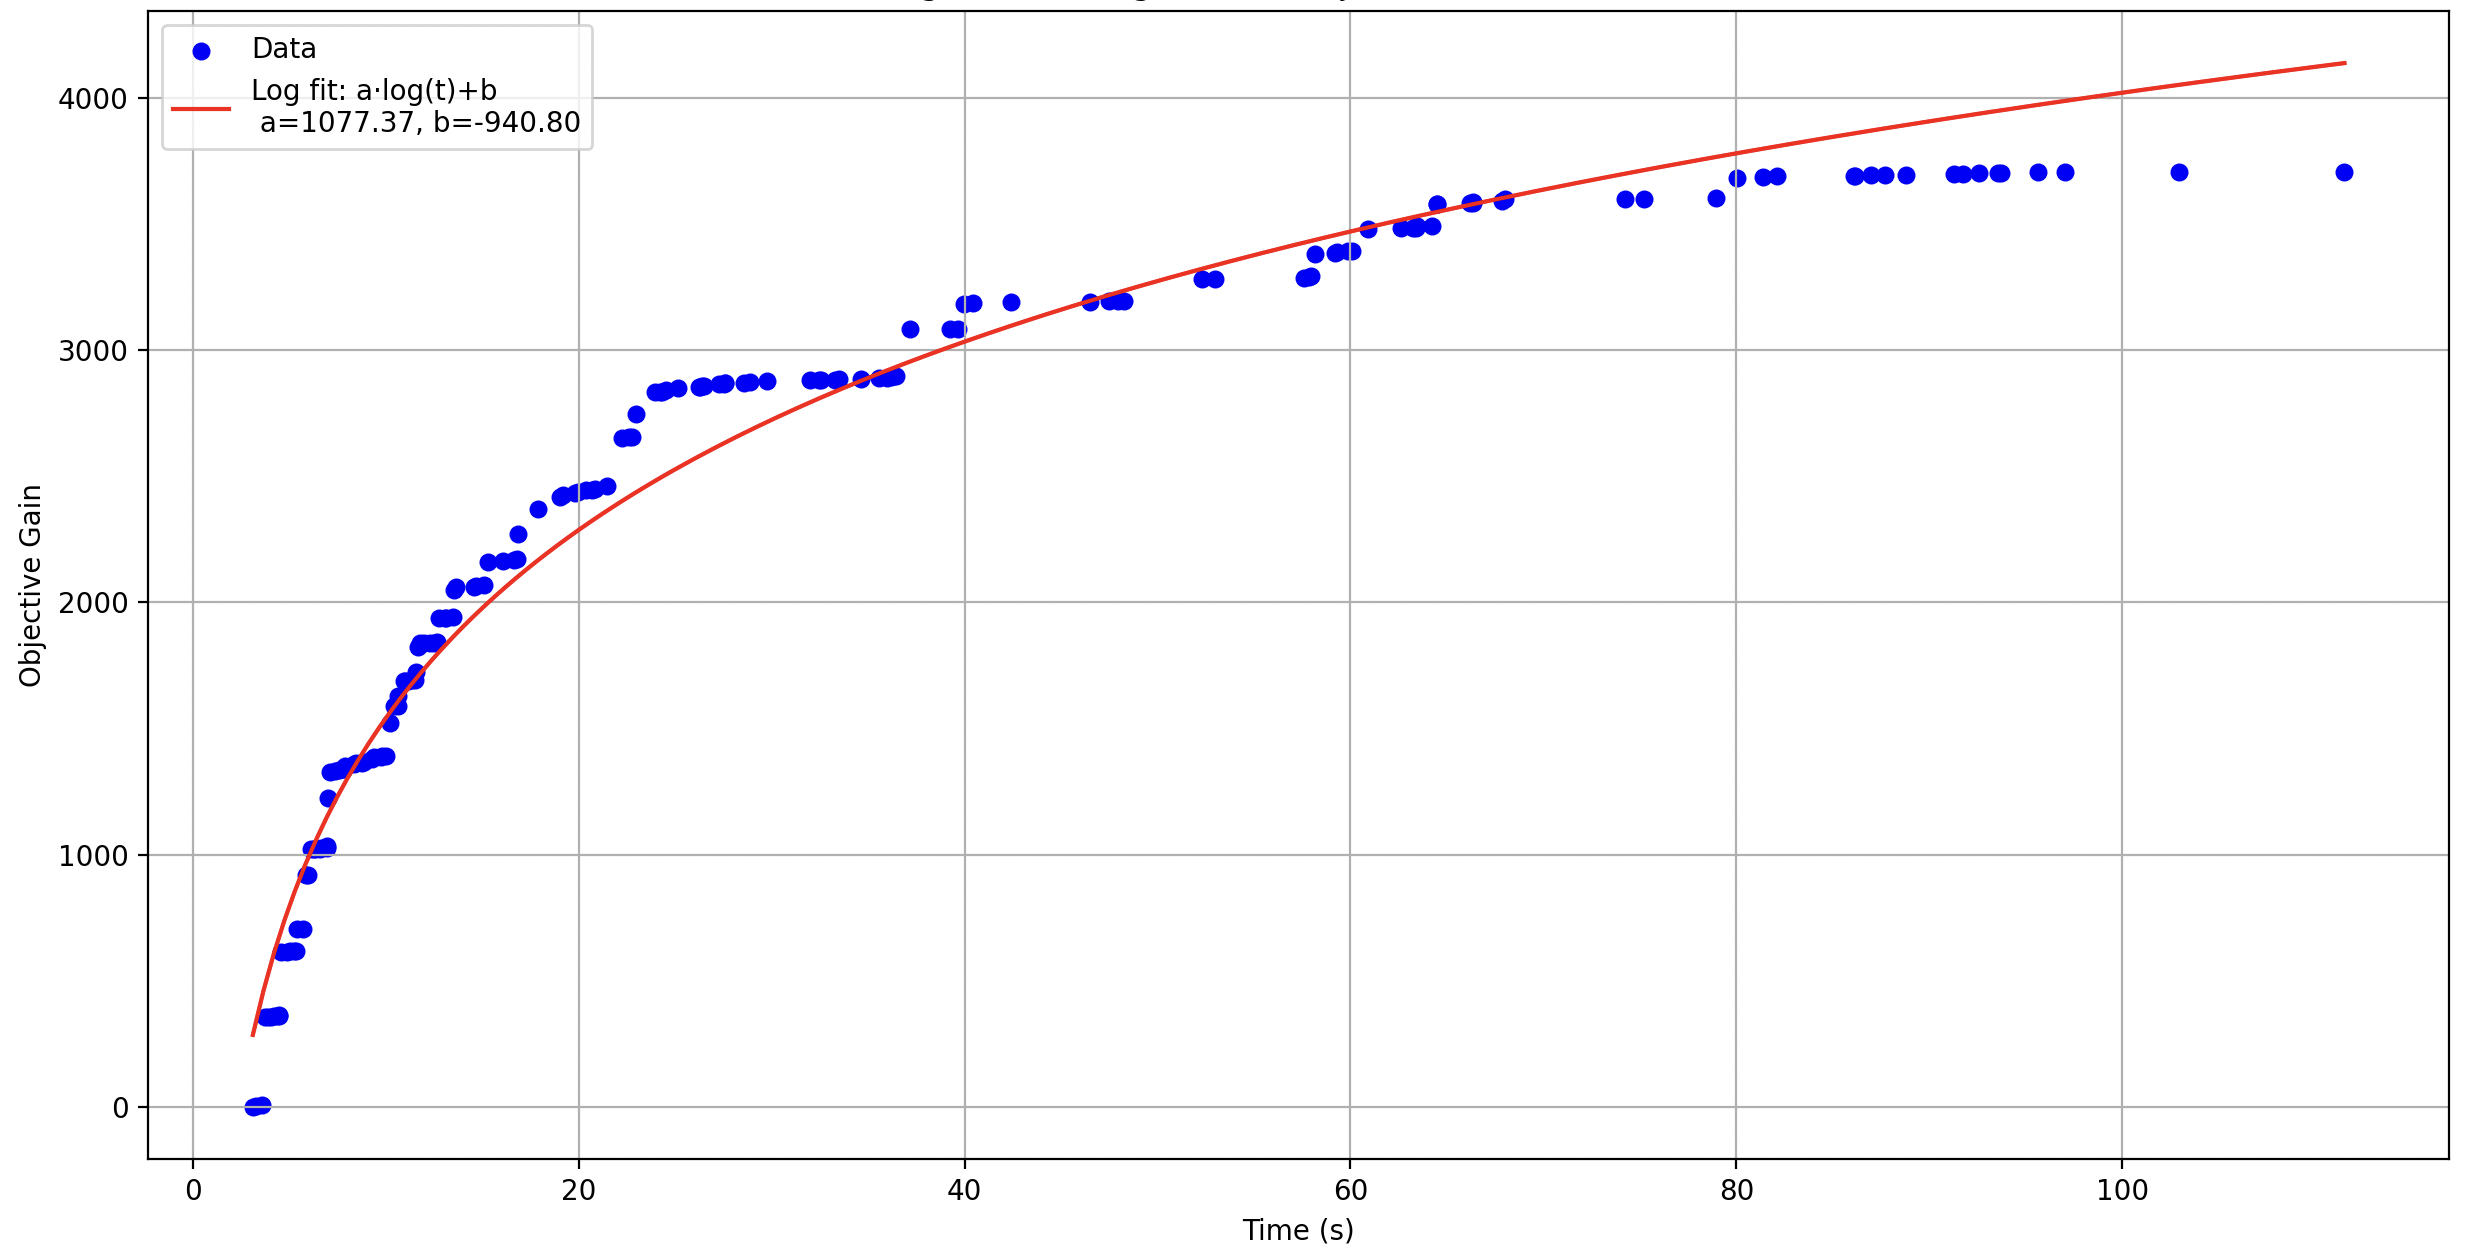
\includegraphics[width=0.75\textwidth]{plot1.png}
  \caption{Objective gain versus time with logarithmic fit (Full instance, 120 s cap).}
  \label{fig:obj-progression}
\end{figure}

We inserted calls to \texttt{solver.Logging()} each time a new incumbent was found, recording both the timestamp and the composite objective value. After collecting these data points, we computed the objective gain by subtracting each incumbent from the initial best and then used SciPy’s \texttt{curve\_fit} to fit a logarithmic function of the form \(g(t)=a\ln(t)+b\). In the resulting plot, the horizontal axis represents wall‐clock time in seconds since the first feasible solution, and the vertical axis shows the objective gain. The fitted parameters \(a\) and \(b\) quantify how quickly the solver closes the gap: a larger \(a\) indicates faster improvements early on, while \(b\) shifts the entire curve vertically. If no new incumbent appears for more than 10 seconds, the solver continues exploring without reporting minor improvements, which manifests as plateaus in the gain curve. 



\subsection{Final Solution Evaluation}

Table~\ref{tab:full‐metrics} presents a concise summary of the key metrics for the full instance (45 teams, 8 main fields with 28 subfields, 130 requests) after running CP–SAT for 120 s.

\begin{table}[h]
  \centering
  \def\arraystretch{1.3}
  \begin{tabularx}{0.75\textwidth}{l X}
    \hline
    \textbf{Average longest‐chain}  & $1.60$ consecutive days per team \\
    \textbf{Average year gap}       & $1.69$ years per co‐located session \\
    \textbf{Ideal adjacency count}  & $34/45$ teams \\
    \hline
  \end{tabularx}
  \caption{Key outcomes for the full instance (120 s cap).}
  \label{tab:full‐metrics}
\end{table}

On average, each team’s longest run of consecutive training days is approximately 1.60 days, which means that most squads never train more than two days in a row. This level of spacing ensures adequate rest and aligns well with typical club expectations. Likewise, the mean age difference of 1.69 years among teams sharing a field on the same day indicates that most sessions are scheduled with closely matched age categories. In practice, clubs often tolerate a 2–3 year spread when demand peaks, so achieving an average under 2 years signifies strong co‐location performance.

Adjacency patterns were judged according to whether a team’s sessions match one of the following: a single session (always ideal), two sessions on non‐consecutive days, exactly \{Mon, Wed, Fri\} for three sessions, or exactly \{Mon, Tue, Thu, Fri\} for four sessions. By these criteria, 34 out of 45 teams attain an “ideal” pattern, meaning over 75\% follow the preferred weekly spacing despite high field utilisation. The remaining 11 teams have non‐ideal spacing only because there was no alternative slot available, not due to modeling shortcomings.

Although the solver did not close the optimality gap, approximately 12\%, the near‐100\% utilisation of available slots suggests that further improvements would require altering session requests or extending availability. From the club’s perspective, the schedule produced is immediately deployable: it balances training load, minimizes age disparities on shared pitches, and satisfies the majority of ideal spacing preferences. Any marginal gains would involve trade‐offs, such as later evening sessions or weekend reallocations that may not be practical under current constraints. It is evident from the evaluated solution and the gain curve in figure 5 that, in practical settings, the solver experiences rapidly diminishing returns after the initial search period, further runtime yields only marginal objective improvements, which do not justify the additional computational expense.

\section{Discussion}

The analysis presented in the previous section provides strong empirical evidence for the effectiveness of constraint programming using the CP-SAT solver in solving complex field scheduling problems. This discussion critically examines the solution method, drawing explicitly on performance metrics and model behaviour. Particular attention is given to scalability, convergence dynamics, and the modelling trade-offs introduced by lexicographic multi-objective optimisation.

\vspace{0.5em}
\vspace{0.5em}
\subsection{Solver performance and scalability}

As Tables~\ref{tab:first‐feasible} and \ref{tab:solver-summary} demonstrate, our CP–SAT prototype exhibits fast convergence even under near‐saturation conditions typical of a local Danish Copenhagen-based club: the small instance yields a first feasible schedule in 0.41 s, the medium instance in 1.66 s, and the full instance in 3.61 s. Likewise, finding and proving optimality for the small and medium instances takes under 8 s and 42 s respectively, while the full instance reaches a high‐quality feasible solution within the 120 s cap, albeit with a 12.4 percent optimality gap.
\\
\\
Importantly, the observed runtime growth is weaker than the growth in our model’s Boolean decision variables \(y_{r,f,d}\).  These indicators number approximately \(40\times8\times5\approx1{,}600\) in the small instance but \(130\times28\times5\approx18{,}200\) in the full instance, an \(11\times\) increase,  yet the time to first feasible solution rises by only about \(9\times\).  Fitting a simple power law to these data yields an exponent of roughly \(0.9\) in the Boolean‐variable count meaning sub‐linear scaling, and about \(1.85\) in the number of requests, i.e.\ sub‐quadratic scaling.
\\
\\
Looking ahead, if one were to double club size, the Boolean count would double but, under \(T\propto m^{0.9}\), runtime would grow by only \(2^{0.9}\approx1.9\times\), far below the \(4\times\) blow‐up of a purely quadratic algorithm.  Combined with CP–SAT’s multi‐threaded search and its global constraints that yield aggressive pruning, this suggests that even moderately larger clubs remain well within acceptable solve‐time budgets. For typical Danish grassroots clubs, approximately ≤50 teams and ≤10 main fields, solve times of a few seconds up to under two minutes are easily achievable on commodity hardware. 
\vspace{0.5em}
\subsection{Effectiveness and limitations of multi-objective optimisation}

When introducing both soft objectives, (O1) minimising the longest chain of consecutive training days per team, and (O2) promoting co-location among age-similar teams, solver performance remained robust in smaller scenarios. For both the small and medium instances, CP-SAT found and verified optimal solutions in under 42 seconds.

However, in the full instance, the solver failed to close the optimality gap within the 120-second time cap, reporting a best-known objective value of 7\,375 against a lower bound of 6\,460, i.e., a 12.4\% gap. Despite this, qualitative metrics showed strong domain alignment: 34 out of 45 teams achieved ideal training spread (non-consecutive or evenly spaced sessions), and the average year gap per co-located session remained at 1.69 years, which is well below the acceptable threshold (2–3 years). These figures indicate that the solver satisfies real-world fairness and preference constraints even without reaching proven optimality.

Still, the outcome underscores a core modelling challenge: the use of a lexicographic weighted-sum objective introduces sensitivity to the chosen weight scalar \( M \). In our implementation, we assigned \( M = 100 \) to ensure that improvements to the primary objective (O1) dominate. This approach guarantees that no co-location benefit (O2) can override a deterioration in adjacency patterns. However, this strategy is brittle. For example, if the maximum possible year-gap sum were underestimated, the solver might inadvertently accept a worse adjacency configuration in favour of minor gains in co-location. Conversely, if \( M \) is set too high, the solver may effectively ignore the secondary objective.

The tension is visible in the full instance: the solver likely prioritised optimising training spread (O1) exclusively for a significant portion of the search, only shifting to O2 improvements once O1 was stable. This two-phase behaviour is appropriate in lexicographic settings, but it also introduces rigidity, adding further objectives (e.g., time-of-day preferences or fairness across weeks) would require additional weighting tiers, further complicating calibration. There is no principled method within CP-SAT to determine appropriate weight magnitudes across heterogeneous objectives. This limitation reduces model generalisability and could lead to non-transparent prioritisation in stakeholder-facing applications.



\vspace{0.5em}
\subsection{Applicability to other domains and the role of discreteness}

The modelling principles used in this project, including discrete time slots, finite resource partitions, and explicit constraint definitions, generalise well to domains such as school timetabling, workforce rostering, and hospital shift planning. These settings share key structural properties, such as limited capacity, mutually exclusive assignments, and the need to balance hard feasibility with soft preferences. Given our results, particularly the solver's rapid convergence in tightly constrained instances, similar performance can be expected in these domains, provided the problem remains discretised.

However, many real-world scheduling problems involve continuous or flexible decision spaces. In transport planning, manufacturing, or energy dispatch, resources may vary over time, tasks can begin at arbitrary points, and availability is not aligned with fixed slots. In such cases, the discrete model structure becomes less applicable. Constraint solvers like CP-SAT cannot operate directly over real-valued domains and would require time to be re-discretised, which may increase the model size and reduce solver efficiency.

This highlights a fundamental trade-off. Discrete models, as demonstrated in our case, support strong propagation and expressive global constraints, but depend on artificial segmentation of time and resources. Continuous domains allow for more realistic modelling but often lack the combinatorial structure needed for effective pruning, making them harder to solve efficiently. For example, reducing the time slot granularity from 15 to 5 minutes triples the number of decision points, with limited practical gain in many scenarios.

In domains where time and resources can be naturally represented in discrete units, such as education, sports scheduling, or static staff planning, constraint programming offers a scalable and interpretable solution method. In contrast, problems that require flexible timing, adaptive allocation, or continuous capacity modelling may benefit more from alternative methods such as mixed-integer programming or hybrid heuristics, despite their lower transparency and reduced solver support for complex combinatorial constraints.


\section{Conclusion}

This project has demonstrated that constraint‐based scheduling using Google’s CP–SAT solver provides a powerful and transparent framework for the complex task of allocating divisible football fields to multiple teams under tight temporal and resource constraints. By modelling each training request as an optional interval variable with associated Boolean and integer indicators, and by exploiting global constraints such as \texttt{AddExactlyOne}, \texttt{NoOverlap} and \texttt{AddCumulative}, our prototype finds high‐quality feasible schedules in a matter of seconds, even on near‐saturated instances with full sized, real club data.
\\
\\
Empirical results show sub‐quadratic scaling in both the number of requests and the Boolean decision variables, with first feasible solutions in under 4 s and proven optimality for small and medium instances within 42 s. Multi‐objective optimisation via a lexicographic weighted‐sum minimising longest chains of consecutive training days (\(\mathrm{O1}\)) before maximising co‐location among same‐year teams (\(\mathrm{O2}\)), yields schedules that satisfy 75\% of teams’ ideal spacing patterns and maintain an average age gap below 2 years, despite a 12.4\% optimality gap on the largest instance. Strong propagation and clause learning ensure that even tight schedules are pruned effectively, while the solver’s branch‐and‐bound engine rapidly improves objectives according to a logarithmic progression.
\\
\\
However, the lexicographic weighting scheme introduces sensitivity to the choice of the multiplier \(M\) and can complicate calibration when additional soft criteria arise. Moreover, the reliance on discrete time slots limits direct applicability to continuous or highly dynamic scheduling contexts. Future work may explore adaptive weight selection methods, integration of rolling‐horizon updates for dynamic requests, or hybrid approaches combining CP–SAT with heuristic repair to better handle continuous time domains.
\\
In summary, our case study confirms that CP–SAT is a scalable, interpretable, and practically deployable tool for grassroots sports scheduling and similar combinatorial planning problems. The methodologies and modelling patterns presented here can be readily adapted to other domains such as school timetabling or workforce rostering where discrete resources, hierarchical allocations, and soft preferences play a central role.




\section{links and resources}
\url{https://developers.google.com/optimization/reference}
\\
\\
\url{https://or-tools.github.io/docs/pdoc/ortools/sat/python/cp_model.html}
\\
\\
\url{https://github.com/d-krupke/cpsat-primer.git}

\section{AI Deklaration}



\includepdf[pages=-]{AI-deklaration-DK.pdf}


\end{document}

